\documentclass[11pt,notheorems,aspectratio=169]{beamer}

% Copyright (c) 2022 by Lars Spreng
% This work is licensed under the Creative Commons Attribution 4.0 International License.
% To view a copy of this license, visit http://creativecommons.org/licenses/by/4.0/
% or send a letter to Creative Commons, PO Box 1866, Mountain View, CA 94042, USA.

%~~~~~~~~~~~~~~~~~~~~~~~~~~~~~~~~~~~~~~~~~~~~~~~~~~~~~~~~~~~~~~~~~~~~~~~~~~~~~~
% Add your packages and commands to this file
%~~~~~~~~~~~~~~~~~~~~~~~~~~~~~~~~~~~~~~~~~~~~~~~~~~~~~~~~~~~~~~~~~~~~~~~~~~~~~~

% Fonts / encoding
\usepackage[T1]{fontenc}
\usepackage[utf8]{inputenc}
\RequirePackage[scaled]{helvet} % sans-serif slides

% Theme
\usepackage{styles/elegantmacros}
\usefolder{styles}
\usetheme[style=lecture]{elegant}

\newcommand{\makepart}[1]{%
	\part{#1}\frame{\partpage}
}

%~~~~~~~~~~~~~~~~~~~~~~~~~~~~~~~~~~~~~~~~~~~~~~~~~~~~~~~~~~~~~~~~~~~~~~~~~~~~~~
% Tables / figures
%~~~~~~~~~~~~~~~~~~~~~~~~~~~~~~~~~~~~~~~~~~~~~~~~~~~~~~~~~~~~~~~~~~~~~~~~~~~~~~
\usepackage{graphicx}
\usepackage{booktabs}
\usepackage{colortbl}
\usepackage{ragged2e}
\usepackage{schemabloc}
\usepackage{caption}
\usepackage{subcaption}
\usepackage{tabularx}
\usepackage{array}
\usepackage{multirow}
\usepackage{wrapfig}
\usepackage{pgfplots}
\usepackage{adjustbox}
\usepackage{environ}
\pgfplotsset{compat=1.18}

\RequirePackage[%
natbib=true,
backend=biber,
style=apa,
isbn=false,
url=false,
uniquename=false
]{biblatex}
\addbibresource{msc-nlp-therapy-speak.bib}

\newcolumntype{Y}{>{\centering\arraybackslash}X}

%~~~~~~~~~~~~~~~~~~~~~~~~~~~~~~~~~~~~~~~~~~~~~~~~~~~~~~~~~~~~~~~~~~~~~~~~~~~~~~
% TikZ
%~~~~~~~~~~~~~~~~~~~~~~~~~~~~~~~~~~~~~~~~~~~~~~~~~~~~~~~~~~~~~~~~~~~~~~~~~~~~~~
\usepackage{tikz}
\usetikzlibrary{shapes,arrows,positioning,fit,backgrounds}

\tikzstyle{decision} = [diamond, draw, fill=blue!20,
text width=7em, text badly centered, inner sep=0pt, minimum height=4em]
\tikzstyle{block} = [rectangle, draw, fill=blue!20,
text width=8.8em, text centered, rounded corners, minimum height=4.0em]
\tikzstyle{block2} = [rectangle, draw, fill=yellow!20,
text width=9.5em, text centered, rounded corners, minimum height=4.0em]
\tikzstyle{line} = [draw, -latex']
\tikzstyle{cloud} = [draw, ellipse, fill=red!20,
minimum width=7.6em, minimum height=4.0em, text centered]
\tikzstyle{note} = [rectangle, draw, dashed, rounded corners, fill=gray!10,
text width=13.2em, text centered, minimum height=3em]

\makeatletter
\newsavebox{\measure@tikzpicture}
\NewEnviron{scaletikzpicturetowidth}[1]{%
	\def\tikz@width{#1}%
	\def\tikzscale{1}%
	\begin{lrbox}{\measure@tikzpicture}%
		\BODY
	\end{lrbox}%
	\pgfmathparse{#1/\wd\measure@tikzpicture}%
	\edef\tikzscale{\pgfmathresult}%
	\BODY
}
\makeatother

%~~~~~~~~~~~~~~~~~~~~~~~~~~~~~~~~~~~~~~~~~~~~~~~~~~~~~~~~~~~~~~~~~~~~~~~~~~~~~~
% Maths
%~~~~~~~~~~~~~~~~~~~~~~~~~~~~~~~~~~~~~~~~~~~~~~~~~~~~~~~~~~~~~~~~~~~~~~~~~~~~~~
\RequirePackage{textcomp}
\RequirePackage{amsmath}
\RequirePackage{amsthm}
\RequirePackage{mathtools}

\DeclareMathOperator*{\argmax}{arg\,max}
\DeclareMathOperator*{\argmin}{arg\,min}

\setbeamertemplate{theorems}[numbered]

\theoremstyle{definition}
\newtheorem{fact}{Fact}[section]
\newtheorem{examp}{Example}[section]

\theoremstyle{plain}
\newtheorem{definition}{Definition}[section]
\newtheorem{proposition}{Proposition}
\newtheorem{theorem}{Theorem}
\newtheorem{assumption}{Assumption}

\providecommand{\H}{\mathscr{H}}
\providecommand{\E}{\mathbb{E}}

\makeatletter
\def\munderbar#1{\underline{\sbox\tw@{$#1$}\dp\tw@\z@\box\tw@}}
\makeatother

\title[Interim Progress]{Therapy-speak in General Web Discourse}
\subtitle{ADHD and Autism over Time in Common Crawl}
\author[Jakob]{Jakob Lütkemeier}
\institute{M.Sc. Applied Social Data Science \\ Trinity College Dublin}
\date{MSc Dissertation Interim Presentation}

\begin{document}
	
	{
		\setbeamertemplate{footline}{}
		\begin{frame}
			\titlepage
			\vspace{-0.4em}
			\begin{alertblock}{Research question}
				How have ADHD- and autism-related terms changed in \textbf{prominence}, \textbf{meaning}, and \textbf{framing} over roughly the last decade?
			\end{alertblock}
		\end{frame}
	}
	\addtocounter{framenumber}{-1}
	
	\section{Motivation and Framework}
	
	
	\begin{frame}{Why this topic, and why now?}
		\begin{block}{Why this matters}
			\begin{itemize}
				\item Mental-health language is no longer confined to the therapy room
				\item That openness is, first and foremost, a good thing
				\item But another side of the coin may be \textbf{semantic drift}
				\item Mis- and overuse can blur meanings and reduce access to the words people actually need
				\item ADHD and autism seem especially salient cases
			\end{itemize}
		\end{block}
		
		\vspace{0.35em}
		
		\begin{alertblock}{Aim}
			Move beyond anecdotes toward large-scale evidence
		\end{alertblock}
	\end{frame}
	
	\begin{frame}{What kinds of change am I studying?}
		\begin{columns}[T,onlytextwidth]
			\column{0.70\textwidth}
			\begin{center}
				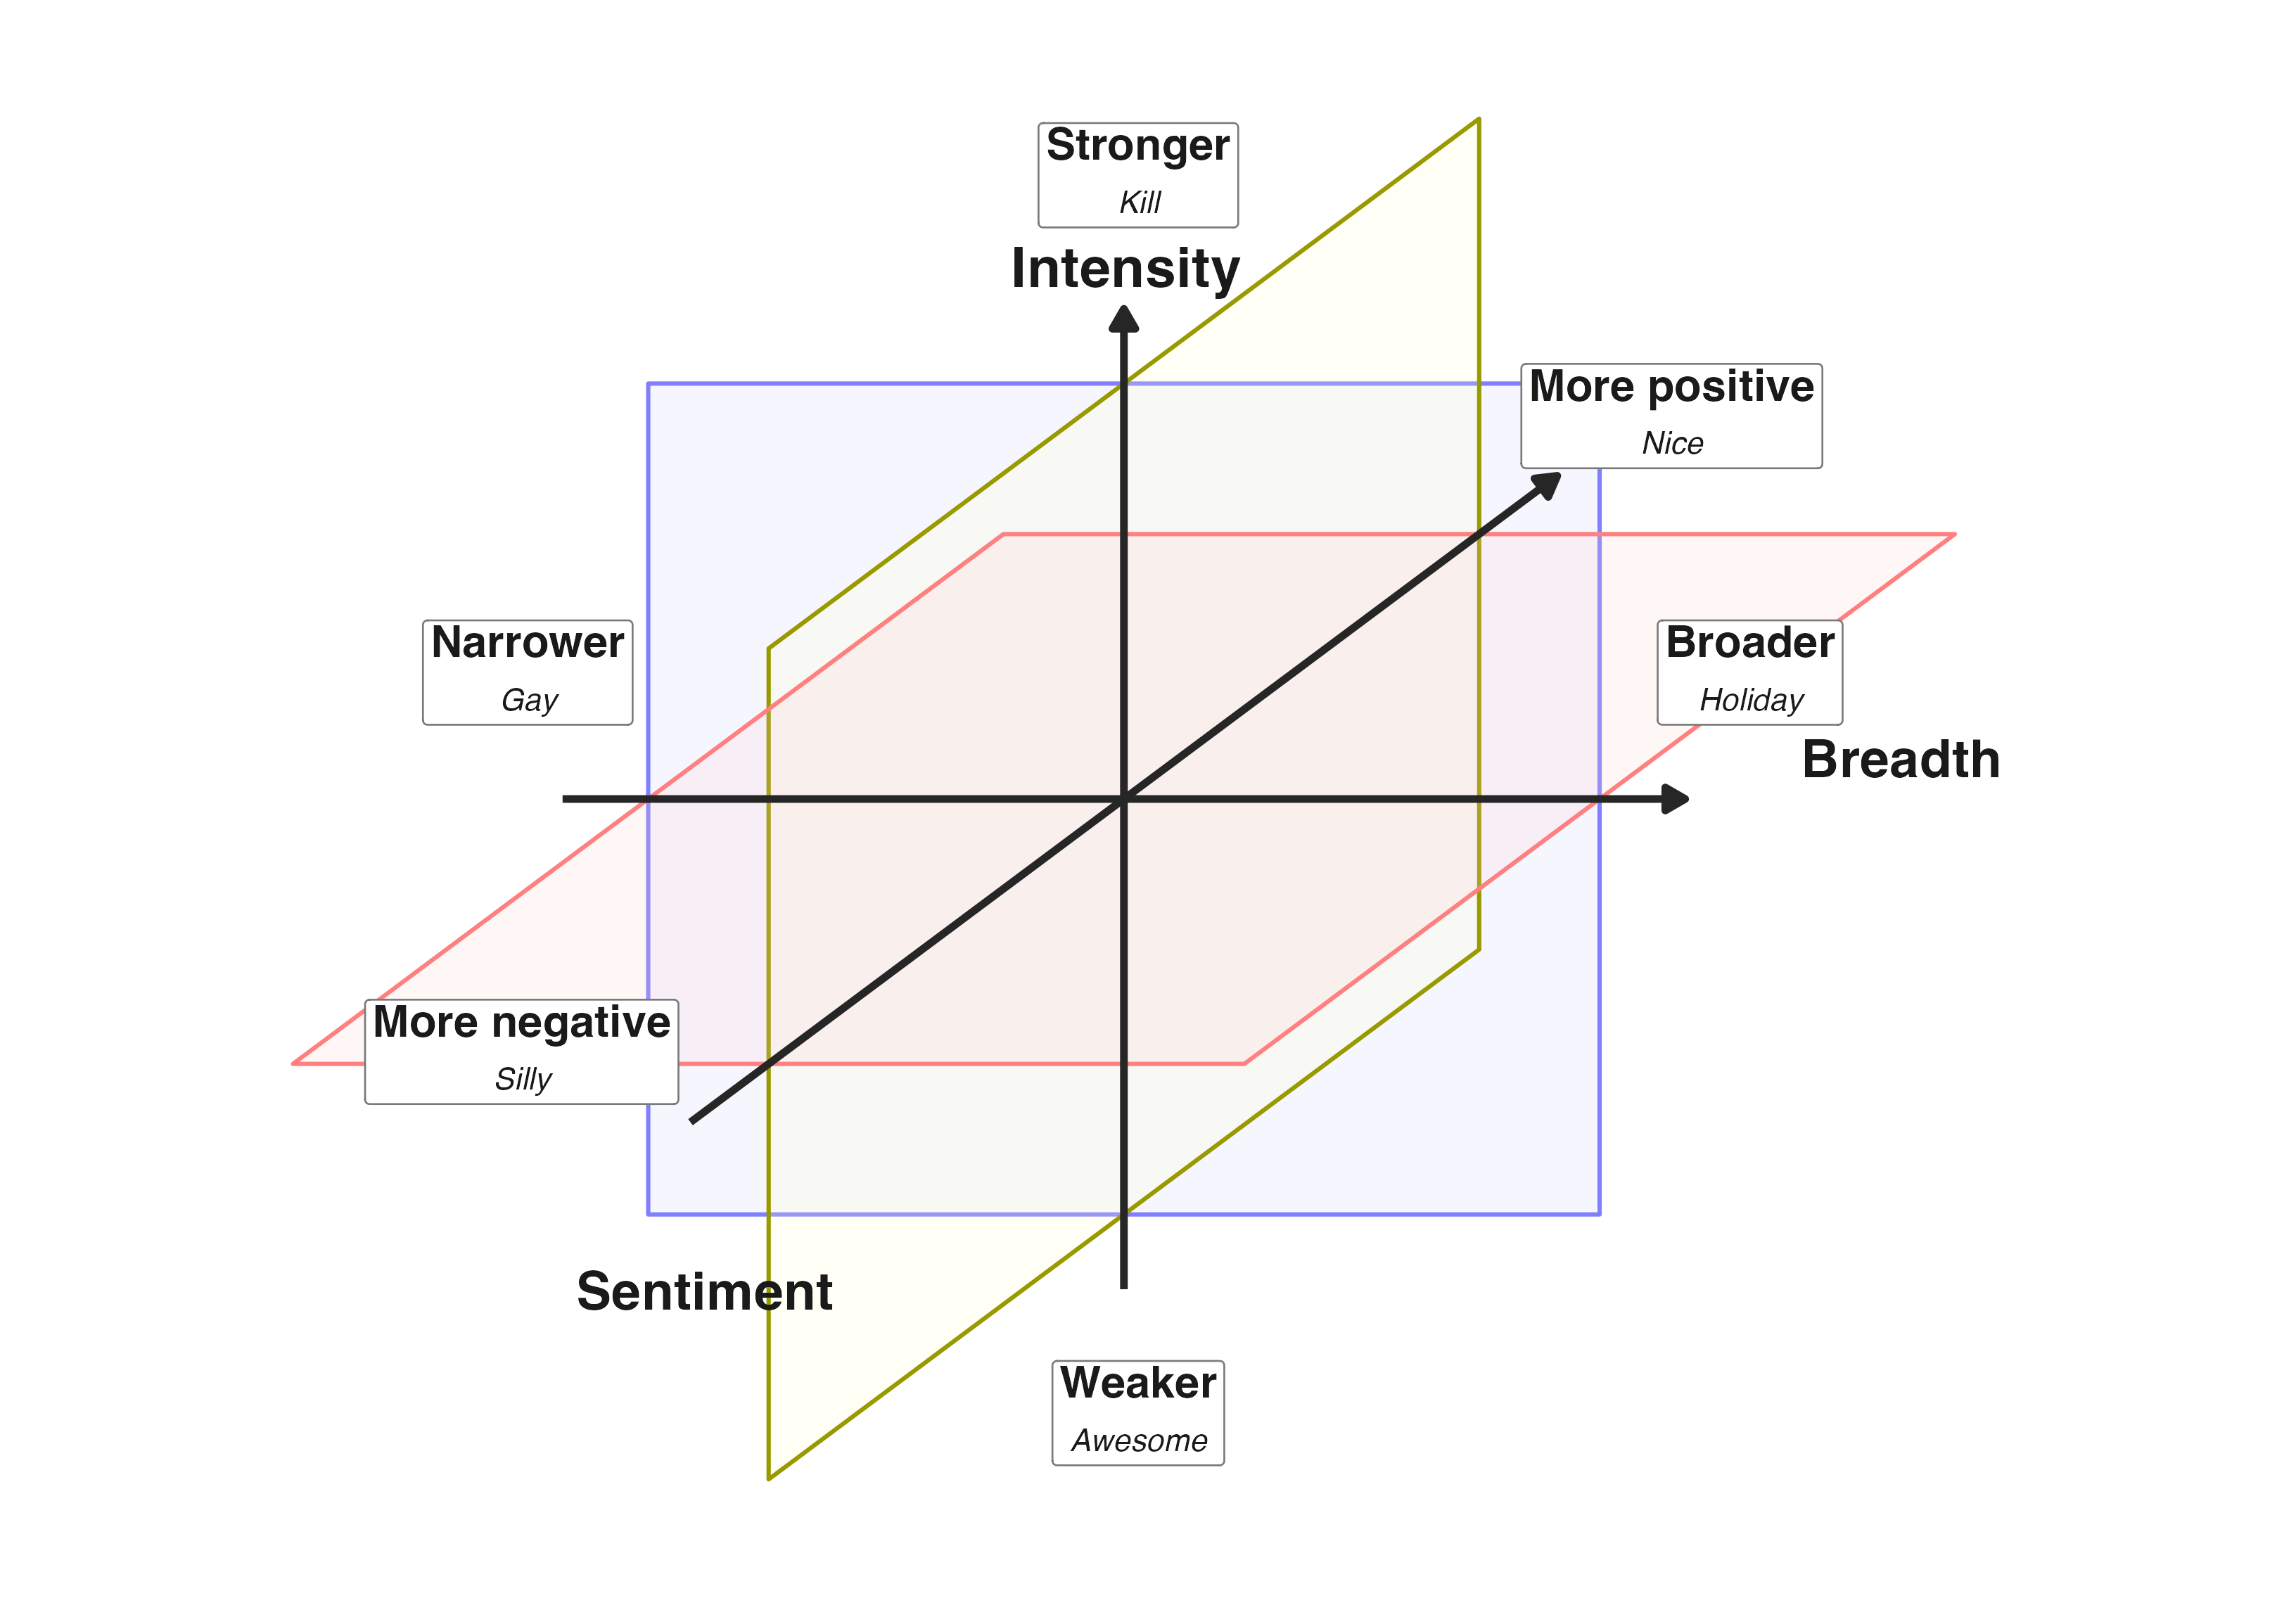
\includegraphics[width=\linewidth]{semantic_drift_framework_final.png}
			\end{center}
			
			\column{0.27\textwidth}
			\begin{block}{\small Other measures of change}
				\textbf{Salience}\\
				\small Frequency of use over time
				
				\vspace{0.9em}
				
				\textbf{Thematic framing}\\
				\small Topics and contexts of use
			\end{block}
		\end{columns}
	\end{frame}
	
	\begin{frame}{How this becomes measurable}
		\begin{block}{From concept to measure}
			\small
			\renewcommand{\arraystretch}{1.25}
			\begin{tabularx}{\linewidth}{>{\bfseries}p{0.18\linewidth} p{0.24\linewidth} X}
				\toprule
				Concept & Measure & What I look at \\
				\midrule
				Salience & yearly mention rates & how often ADHD/autism terms appear over time \\
				Intensity & collocate arousal / severity & whether surrounding language becomes weaker or stronger \\
				Sentiment & collocate valence & whether surrounding language becomes more positive or negative \\
				Breadth & contextual dispersion & how narrowly or broadly terms are used across contexts \\
				Thematic framing & topic modelling over time & which kinds of topics and associations cluster around the terms \\
				\bottomrule
			\end{tabularx}
		\end{block}
	\end{frame}
	
	\begin{frame}{Why Common Crawl?}
		\begin{columns}[T,onlytextwidth]
			\column{1.0\textwidth}
			\begin{columns}[T,onlytextwidth]
				\column{0.32\textwidth}
				\begin{exampleblock}{\centering \Large 10+ PiB}
					\centering
					\small archive size
				\end{exampleblock}
				\column{0.32\textwidth}
				\begin{exampleblock}{\centering \Large 300B+}
					\centering
					\small web pages
				\end{exampleblock}
				\column{0.32\textwidth}
				\begin{exampleblock}{\centering \Large since 2007}
					\centering
					\small historical depth
				\end{exampleblock}
			\end{columns}
			
			\vspace{0.9em}
			
			\begin{center}
				\large General web discourse at a scale suitable for diachronic analysis
			\end{center}
		\end{columns}
	\end{frame}
	
	\begin{frame}{The challenge with Common Crawl}
		\begin{alertblock}{Main challenge}
			Getting \textbf{clean text} in a way that is \textbf{computationally feasible}
		\end{alertblock}
		
		\vspace{0.6em}
		
		\begin{columns}[T,onlytextwidth]
			\column{0.47\textwidth}
			\begin{block}{Common Crawl data layers}
				\small
				\textbf{WET}\\
				extracted plaintext only
				
				\vspace{0.6em}
				
				\textbf{WARC}\\
				complete web-page data, including HTML and metadata
			\end{block}
			
			\column{0.49\textwidth}
			\begin{block}{Typical boilerplate examples}
				\begin{itemize}
					\item navigation menus
					\item cookie banners
					\item accessibility widgets
				\end{itemize}
			\end{block}
		\end{columns}
	\end{frame}
	
	\section{Collection Strategy}
	
	\begin{frame}{Corpus collection pipeline}
		\begin{center}
			\resizebox{\textwidth}{!}{%
				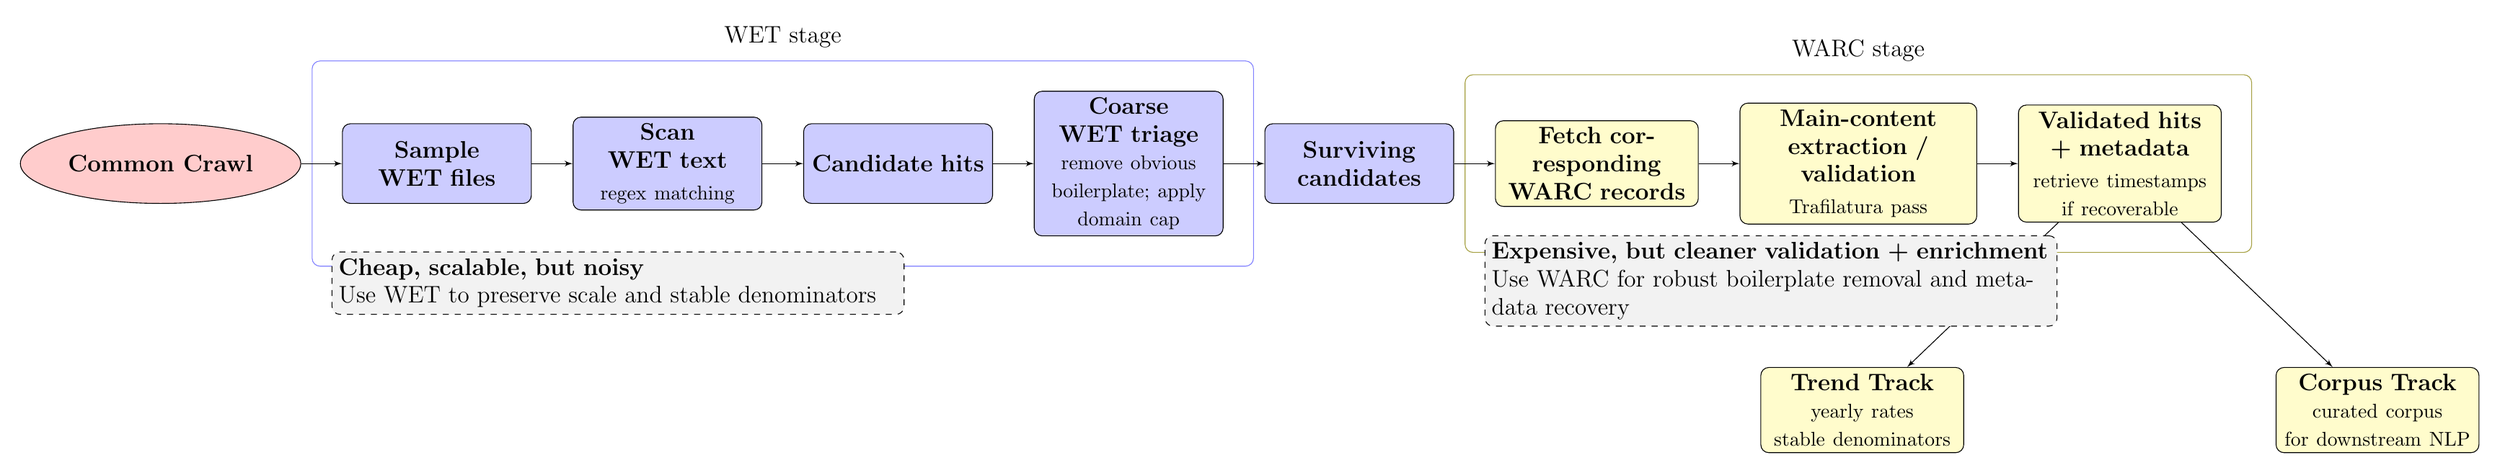
\begin{tikzpicture}[node distance = 1.05cm and 0.72cm, auto, every node/.style={font=\large}]
					
					% Main pipeline nodes
					\node [cloud] (cc) {\textbf{Common Crawl}};
					\node [block, right=of cc] (wet) {\textbf{Sample}\\\textbf{WET files}};
					\node [block, right=of wet] (scan) {\textbf{Scan WET text}\\[0.15em]\normalsize regex matching};
					\node [block, right=of scan] (cand) {\textbf{Candidate hits}};
					\node [block, right=of cand] (triage) {\textbf{Coarse WET triage}\\[0.15em]\normalsize remove obvious\\boilerplate; apply domain cap};
					\node [block, right=of triage] (survive) {\textbf{Surviving}\\\textbf{candidates}};
					\node [block2, right=of survive] (warc) {\textbf{Fetch corresponding}\\\textbf{WARC records}};
					\node [block2, text width=11.2em, right=of warc] (validate) {\textbf{Main-content}\\\textbf{extraction / validation}\\[0.15em]\normalsize Trafilatura pass};
					\node [block2, right=of validate] (valid) {\textbf{Validated hits}\\\textbf{+ metadata}\\[0.15em]\normalsize retrieve timestamps if recoverable};
					
					% Output branches
					\node [block2, below left=2.55cm and 0.95cm of valid] (trend) {\textbf{Trend Track}\\[0.15em]\normalsize yearly rates\\stable denominators};
					\node [block2, below right=2.55cm and 0.95cm of valid] (corpus) {\textbf{Corpus Track}\\[0.15em]\normalsize curated corpus\\for downstream NLP};
					
					% Edges
					\path [line] (cc) -- (wet);
					\path [line] (wet) -- (scan);
					\path [line] (scan) -- (cand);
					\path [line] (cand) -- (triage);
					\path [line] (triage) -- (survive);
					\path [line] (survive) -- (warc);
					\path [line] (warc) -- (validate);
					\path [line] (validate) -- (valid);
					\path [line] (valid) -- (trend);
					\path [line] (valid) -- (corpus);
					
					% Background grouping boxes
					\begin{scope}[on background layer]
						\node [draw=blue!50, rounded corners, inner sep=15pt,
						fit=(wet) (triage),
						label={[font=\large, yshift=0.3em]above:WET stage}] (wetstage) {};
						\node [draw=yellow!60!black, rounded corners, inner sep=15pt,
						fit=(warc) (valid),
						label={[font=\large, yshift=0.3em]above:WARC stage}] (warcstage) {};
					\end{scope}
					
					% Notes
					\node [note, anchor=south west, text width=28em, align=left]
					(wetnote) at ([xshift=0.35cm,yshift=-0.85cm]wetstage.south west)
					{\textbf{Cheap, scalable, but noisy}\\Use WET to preserve scale and stable denominators};
					
					\node [note, anchor=south west, text width=28em, align=left]
					(warcnote) at ([xshift=0.35cm,yshift=-1.3cm]warcstage.south west)
					{\textbf{Expensive, but cleaner validation + enrichment}\\Use WARC for robust boilerplate removal and metadata recovery};
					
				\end{tikzpicture}%
			}
		\end{center}
		
		\vspace{0.15em}
		
		{\small
			\begin{columns}[T,onlytextwidth]
				\column{0.50\textwidth}
				\begin{alertblock}{Current position}
					WET-based screening is working $\rightarrow$ now moving into WARC-based validation/enrichment
				\end{alertblock}
				\column{0.50\textwidth}
				\begin{block}{WET stage pilot test results}
					\begin{itemize}
						\item \textasciitilde157k documents scanned
						\item 728 candidate hits (0.46\%)
						\item 596 surviving candidates post WET triage
					\end{itemize}
				\end{block}
		\end{columns}}
	\end{frame}
	
	\begin{frame}{Next steps, risks, and what success looks like}
		\begin{columns}[T,onlytextwidth]
			\column{0.32\textwidth}
			\begin{block}{Next}
				\begin{itemize}
					\item WARC-based full-fledged boilerplate removal
					\item timestamp / metadata enrichment
					\item then scale to the full diachronic dataset
				\end{itemize}
			\end{block}
			
			\column{0.32\textwidth}
			\begin{block}{Main risks}
				\begin{itemize}
					\item residual boilerplate noise
					\item incomplete timestamps
					\item computational cost
				\end{itemize}
			\end{block}
			
			\column{0.32\textwidth}
			\begin{exampleblock}{Success looks like}
				\begin{itemize}
					\item stable yearly trend estimates
					\item clean(er) validated corpus
				\end{itemize}
			\end{exampleblock}
		\end{columns}
	\end{frame}
	
\end{document}